\documentclass{article}
\usepackage[utf8]{inputenc}
\usepackage{polski}
\usepackage{fancyhdr}
\usepackage{multirow}
\usepackage{graphicx}



\fancyhead[L]{}
\fancyhead[R]{}
\fancyfoot[L]{Mateusz Redzimski}
\fancyfoot[C]{\thepage}
\fancyfoot[R]{Środowisko Programisty}

\title{Poważne teksty łacińskie oraz inne ważne informacje.}
\author{Mateusz Redzimski}


\markright{Mateusz Redzimski}

\begin{document}

\maketitle
\newpage
\pagestyle{fancy}
\tableofcontents
\listoftables
\listoffigures
\newpage
\section{Pierwszy poważny tekst łaciński}
\qquad
Lorem ipsum dolor sit amet, consectetur adipiscing elit. Mauris laoreet efficitur pulvinar. Sed condimentum leo eget augue condimentum fringilla. Fusce euismod, purus vitae efficitur ultricies, elit leo facilisis nisi, ornare congue libero orci ut mauris. Pellentesque pharetra nunc eget tincidunt molestie. Nullam fermentum lorem eu varius fermentum. Pellentesque at hendrerit ex. Donec ac augue ex. Cras quis sagittis mi.

\section{Drugi poważny tekst łaciński}
\qquad
 Lorem ipsum dolor sit amet, consectetur adipiscing elit. Aliquam purus elit, mattis ut libero sit amet, bibendum dignissim nulla. Sed sit amet quam tempor nisi aliquet sodales at ac odio. Vestibulum eget mauris imperdiet, vestibulum sapien nec, finibus erat. Nulla a metus nec turpis porttitor vehicula sit amet in sapien. Maecenas sit amet neque in nisi imperdiet tristique. Pellentesque nisi magna, convallis in finibus et, commodo non neque. Nullam auctor risus vel augue tristique aliquam. Sed sollicitudin augue ut leo congue viverra. Nulla tincidunt tempus diam sit amet sagittis. Aenean molestie nibh in nunc vestibulum scelerisque.

\subsection{ Pierwszy podrozdział drugiego poważnego tekstu łacińskiego}
\qquad
Cras sed felis non metus dignissim iaculis eu in risus. Aliquam mauris mi, bibendum pharetra nunc et, pulvinar dignissim ex. Class aptent taciti sociosqu ad litora torquent per conubia nostra, per inceptos himenaeos. Mauris sodales id elit tincidunt mollis. Sed aliquet metus velit, eget tincidunt ligula facilisis non. Proin semper pretium ornare. Curabitur quis aliquet ante. Nullam aliquam ultricies eros eu semper. In at maximus nisl. Etiam sit amet tellus erat.

\subsection{ Drugi podrozdział drugiego poważnego tekstu łacińskiego}
\qquad
Etiam eu varius ex. Quisque facilisis est consectetur pharetra viverra. Integer quis ultrices augue. Pellentesque nisl odio, laoreet quis euismod vitae, ultrices tristique augue. Quisque sagittis libero ac nisi ultrices tristique. Quisque blandit aliquam suscipit. Praesent non auctor odio. Integer ac sapien felis. Phasellus maximus mollis ligula, in fermentum sem scelerisque nec. Duis nec nunc in nisi ultrices gravida.

\newpage
\section{Tablica matematyczna}

\begin{table}[h!]
  \begin{center}
    \caption{Tablica trygonometryczna.}
    \label{tab:table1}
	\Large
	\renewcommand{\arraystretch}{2}
    \begin{tabular}{|c|c|c|c|c|c|}
	\hline
	\multirow{2}{*}{$\alpha$} & 0° & 30° & 45° & 60° & 90° \\
  	&  0 &$\frac{\pi}{6}$ &$\frac{\pi}{4}$ & $\frac{\pi}{3}$ &$\frac{\pi}{2}$ \\
	\hline
	sin $\alpha$ & 0 & $\frac{1}{2}$ & $\frac{\sqrt{2}}{2}$ & $\frac{\sqrt{3}}{2}$ & 1 \\

	\hline
	cos $\alpha$ & 0 & $\frac{\sqrt{3}}{2}$ & $\frac{\sqrt{2}}{2}$ &  $\frac{1}{2}$ & 1 \\
	\hline
	tg$\alpha$  & 0 &   $\frac{\sqrt{3}}{3}$ & 1 & $\sqrt{3}$ & nie istnieje \\
	\hline
    \end{tabular}
	\renewcommand{\arraystretch}{1}
  \end{center}
\end{table}

\newpage 
\section{Słynne obrazy}

\begin{figure}[h!]
\centering
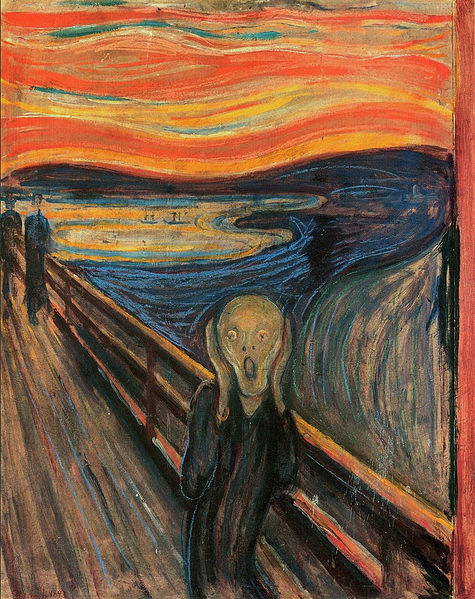
\includegraphics[width=7cm]{studentpodczassesji}
\caption{Krzyk- Edvard munch}
\label{fig:Krzyk}
\end{figure}

\begin{figure}[h!]
\centering
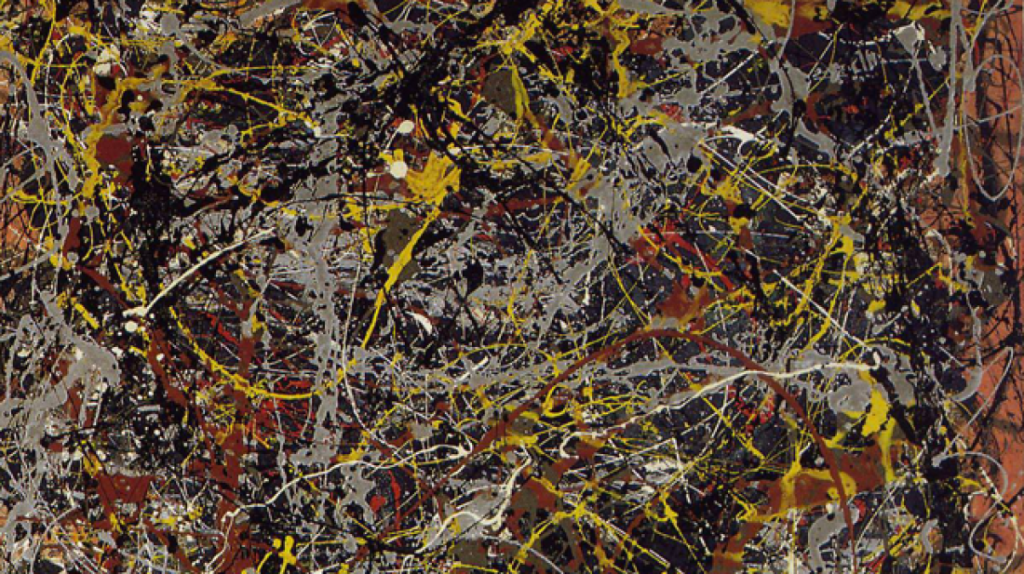
\includegraphics[width=12cm, angle=180]{niktniezauwazyzejestdogorynogamii}
\caption{nr 5, 1948 – Jackson Pollock}
\label{fig:obrazek k}
\end{figure}

\newpage
\section{Najwyżej oceniane filmy na świecie według użytkowników Filmweb}

\begin{enumerate}
\large
  \item The Shawshank Redemption 1994
  \item Intouchables 2011
  \item The Green Mile 1999
  \item The Godfather 1972
  \item 12 Angry Men 1957
  \item Forrest Gump
  \item One Flew Over the Cuckoo's Nest 1975
  \item The Godfather: Part II 1974
  \item Schindler's List 1993
  \item The Lord of the Rings: The Return of the King 2003
\end{enumerate}

\section{Lista owoców które można zjeść}

\begin {itemize}
\large
  \item Jabłko \cite{brown2012apple}
  \item Banan \cite{seymour1993banana}
  \item Mandarynka \cite{sybesma2013mandarin}
  \item Grejpfrut \cite{bailey1998grapefruit}
  \item Mango \cite{mirta1997mango}
  \item Marakuja \cite{zibadi2004passion}
  \item Liczi \cite{menzel1987lychee}
  \item Borówka \cite{chu2011bilberry}
  \item Truskawka \cite{darrow1966strawberry}
  \item Pomidor \cite{just1980tomatoes}
\end {itemize}

\newpage
\section{Cytaty z filmu Killer}
\begin{itemize}
\item "\emph{Co} \textup{ty} \textsc{wiesz} o \textbf{zabijaniu}?! \textsl{Ty} \texttt{stara} \textit{dupa} \textsf{jesteś}"~~ Jerzy Killer 
\item "\tiny Co \scriptsize ty \footnotesize myślisz, \small cwaniaczku?! Że z \large piątego przykazania \Large możesz sobie  \LARGE zrobić spółkę z  \huge ograniczoną  \Huge odpowiedzialnością?!" \normalsize ~~ Komisarz Jerzy Ryba
\end{itemize}



\bibliographystyle{abbrv}
\bibliography{Mojabiblio}

\end{document}
